\documentclass[14pt]{extarticle}
\usepackage[spanish]{babel} 
\usepackage[utf8]{inputenc} %Este es el paquete para que te muestre bien los caracteres latinos
\usepackage[useregional]{datetime2} %paquete para la fecha
\usepackage[a4paper]{geometry} %paquete para el tamaño de hoja
\usepackage{changepage} %paquete para cambiar los márgenes a una sola parte del documento con \begin{adjustwidth} y \end{adjustwidth}
\usepackage{lmodern}
%\usepackage{palatino}
\usepackage{fancyhdr} %para los estilos de hoja, también para los l-rhead, l-rfoot
\usepackage{subcaption}
\usepackage[breaklinks=true]{hyperref} %separa las referencias muy largas en varias lineas
\usepackage[pdftex]{graphicx} %paquete para las imágenes
\usepackage[numbers]{natbib}
\graphicspath{ {images/} }
%\usepackage[final]{pdfpages}
%paquete para incorporar pdfs




\newcommand{\fecha}{\today}
\newcommand{\docker}{Docker\copyright}


\begin{document}


    \begin{titlepage}

        \begin{center}
            
\includegraphics{logoUnpsjb.png}
            \linebreak
            \begin{huge}
                Sistemas Operativos \\ Trabajo Práctico Final \\ \docker{}\\
            \end{huge}
            \vspace*{5mm}
            \rule{10cm}{0.1mm}\\
            \vspace*{3mm}
            \begin{Large}
                Cátedra:\\
                \textbf{Profesor:} Lic. Marcelo Gómez\\
                \vspace*{5mm}
                \textbf{Ayudantes de cátedra:}\\ Lic. Lucy Marticorena\\APU Leandro Luque\\
            \end{Large}
            \vspace*{3mm}
            \rule{10cm}{0.1mm}\\
            \vspace*{5mm}
            \begin{large}
                Alumnos:\\
                SERRUYA ALOISI, Luciano\\
                TOLEDO MARGALEF, Pablo\\
            \end{large}
            \vspace*{5mm}
            \Large\fecha
    \end{center}

    \end{titlepage}

    \clearpage
    \pagestyle{fancy}
    \cfoot{}
    \lhead{TP Final - Docker}
    \rhead{
\includegraphics[scale=0.2]{logoUnpsjb.png}}
    \lfoot{\thepage}
    \rfoot{Luciano Serruya Aloisi, Pablo Toledo Margalef}

    \clearpage
    \tableofcontents
    \clearpage

    \section{Introducción}
        Un buen punto de partida antes de empezar a describir la tecnología \docker{}, sería hacer una breve introducción a la \textbf{virtualización}.

        El sitio de RedHat Inc. describe a la virtualización de la siguiente manera:

        \begin{quote}
            La virtualización es una tecnología que permite crear múltiples ambientes simulados o recursos dedicados a partir de un sistema de hardware. Un software llamado \textit{hypervisor} se conecta directamente con ese hardware y brinda la posibilidad de dividir un sistema en varios entornos separados, distintos y seguros conocidos como \textbf{Máquinas virtuales}. Dichas máquinas se basan el la habilidad del \textit{hypervisor} para abstraer los recursos del hardware y distribuirlos entre las máquinas virtuales acordemente \cite{redhat}
        \end{quote}

        Las tecnologías que permiten la virtualización surgieron en la década del 1960, sin embargo obtuvieron mayor popularidad cuando varias empresas tenían que correr software de distintos fabricantes en máquinas de un fabricante en particular (que sólo permitían correr su software).
        
        Utilizando la virtualización, dichas organizaciones podían correr software de distintos fabricantes usando distintos tipos y versiones de sistemas operativos. De esta forma, los servidores se utilizaban más eficientemente, reduciendo costos de compras, de instalación, mantenimiento, y refrigeración.

        Los recursos que comunmente se virtualizan son los \textbf{servidores}, \textbf{sistemas operativos}, y las \textbf{redes}. 

        Virtualizar servidores sirve para maximizar su rendimiento, logrando así poder atender más solicitudes de clientes y poder usar sus componentes para realizar más funciones.
        Virtualizar sistemas operativos permite tener distintos sistemas operativos corriendo a la vez (por ejemplo, tener una imagen de Windows, y otra de alguna distribución Linux).
        La virtualización de redes reduce los componentes físicos necesarios para crear múltiples redes independientes entre sí.

    \subsection{Máquinas virtuales}
        Como se describió anteriormente, las máquinas virtuales son una \textbf{abstracción de los recursos del hardware}. Son programas que emulan una computadora, dando la sensación de que lo que ejecuta la máquina virtual lo ejecuta directamente sobre el hardware (por ejemplo, la máquina virtual cree que tiene un disco duro de 10GB, mientras que realmente es un archivo más en el filesystem del sistema operativo anfitrión).
        
        La capa intermedia que existe entre la máquina virtual y el hardware real se encarga de crear y administrar los recursos físicos para las distintas instancias de máquinas virtuales que estén corriendo en simultáneo.
        Esta capa intermedia puede correr encima del sistema operativo anfitrión (como por ejemplo VirtualBox, también llamados \textit{Type 2 Hypervisors}), o se puede ejecutar directamente sobre el hardware (\textit{Type 1 Hypervisors}, por ejemplo KVM)\cite{ibm}. Esta última opción logra mejores rendimientos que la primera ya que se elimina una capa intermedia (que sería el sistema operativo anfitrión), siendo el \textit{hypervisor} el anfitrión, y las máquinas virtuales corren encima de él. 

        Esta opción de virtualización consume bastantes recursos de la máquina anfitriona, ya que debe emular el sistema completo, desde los recursos físicos (disco duro, procesador, RAM), hasta el filesystem del sistema operativo huésped.

        \begin{figure}
            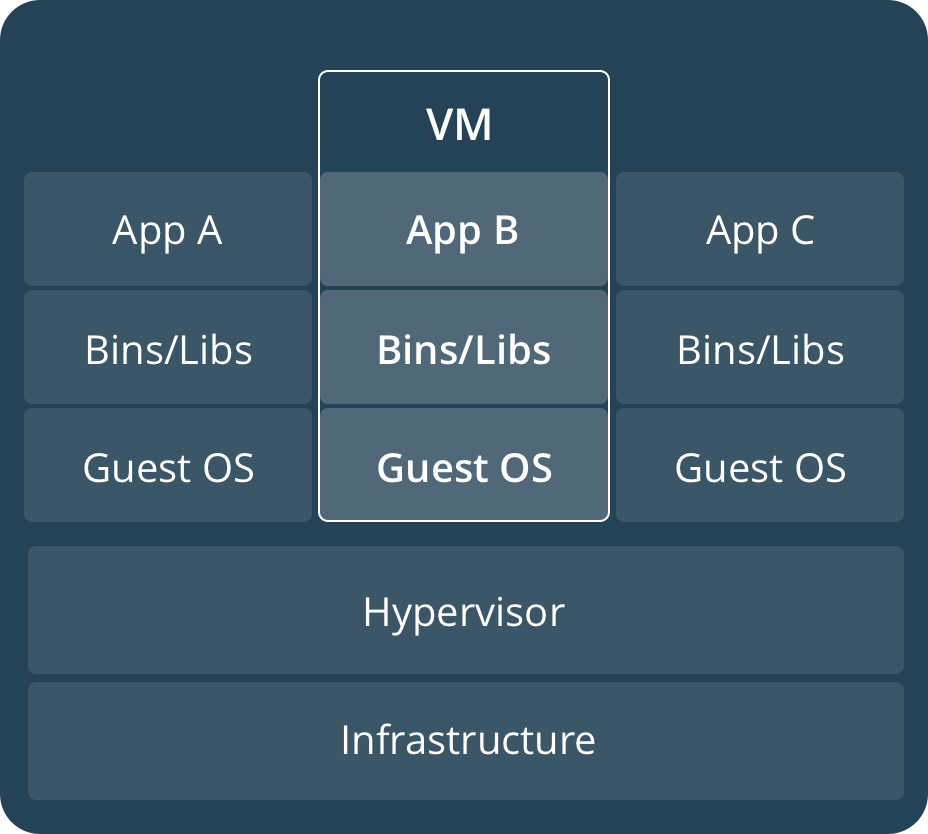
\includegraphics[scale=0.30]{vms.png}
            \caption{Máquinas virtuales sobre \textit{hypervisor}}
        \end{figure}

        \pagebreak


    \subsection{Plataformas de contenedores}
        Por otro lado existen también los \textbf{contenedores}, que el sitio de \docker{} los describe como ``paquete ejecutable liviano y autónomo de una pieza de software que incluye todo lo que necesita para correr: código, librería del sistema, configuraciones''. 
        
        Los contenedores son una abstracción en la capa de la aplicación que aislan el software que se desea ejecutar, armando un pequeño ambiente con las dependencias necesarias para que se ejecute solamente ese código. Esto facilita el trabajo de los desarrolladores, sabiendo que al trabajar y probar su producto en un contenedor, ese mismo contenedor podrá ser puesto en producción con la certeza de que funcionará, evitando incertidumbres que pueden generar intentar de ejecutar el software en distintos sistemas operativos o hardware.
        
        El sistema operativo anfitrión sobre el que corren los contenedores restringe el acceso del contenedor a los recursos físicos, por lo tanto un solo contenedor no podrá consumir todos los recursos del anfitrión. Como todos los contenedores comparten el kérnel del sistema operativo anfitrión, logran que su uso (también llamado \textit{virtualización basada en contenedores}) sea más eficiente que el uso de las máquinas virtuales (donde cada máquina virtual ejecutaba un sistema operativo entero)\\

        \begin{figure}
            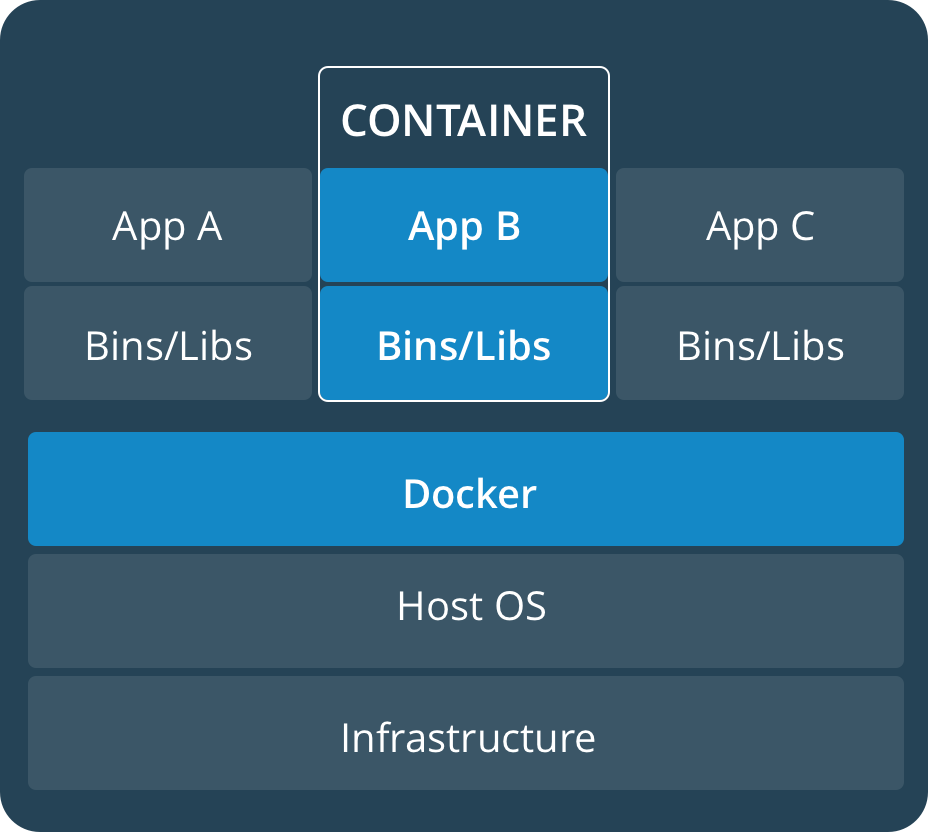
\includegraphics[scale=0.30]{containers.png}
            \caption{Contenedores corriendo sobre la plataforma \docker{}}
        \end{figure}

        \begin{quote}
            La diferencia clave entre los contenedores y las máquinas virtuales es que, mientras el \textit{hypervisor} abstrae un dispositivo entero, los contenedores solo abstraen el kérnel del sistema operativo. \cite{dockerdarnpopular}
        \end{quote}

        Al momento de momento de decidir si usar una máquina virtual o un contenedor para ejecutar una aplicación de forma aislada, no se debe perder de vista el \textbf{alcance} que se espera que tenga la aplicación.\cite{cloudinfrastructure}

        Al ser los contenedores mucho más livianos que las máquinas virtuales (no tienen que correr una instancia del sistema operativo, sólo la aplicación para la cual fueron diseñados), permiten elevar más el nivel de abstracción, logrando tener un contenedor altamente específico para correr una aplicación en particular.  Como práctica general, se mantiene el concepto de tener \textbf{un proceso por contenedor}.

        Las máquinas virtuales tienen un alcance mucho más amplio, permitiendo correr sistemas operativos enteros.  


    \clearpage
    \pagebreak
    \section{¿Qué es \docker{}?}


        \docker{} es una plataforma de contenedores de código abierto creada en el 2013. La premisa de la empresa es que la herramienta que ellos proveen está destinada a eliminar el problema de ``Funciona en mi computadora''\cite{docker}, al empaquetar el ambiente de ejecución de la aplicación en un contenedor (o imagen) y transportar esa imagen de un servidor a otro.


        \begin{figure}[h]
            \centering
            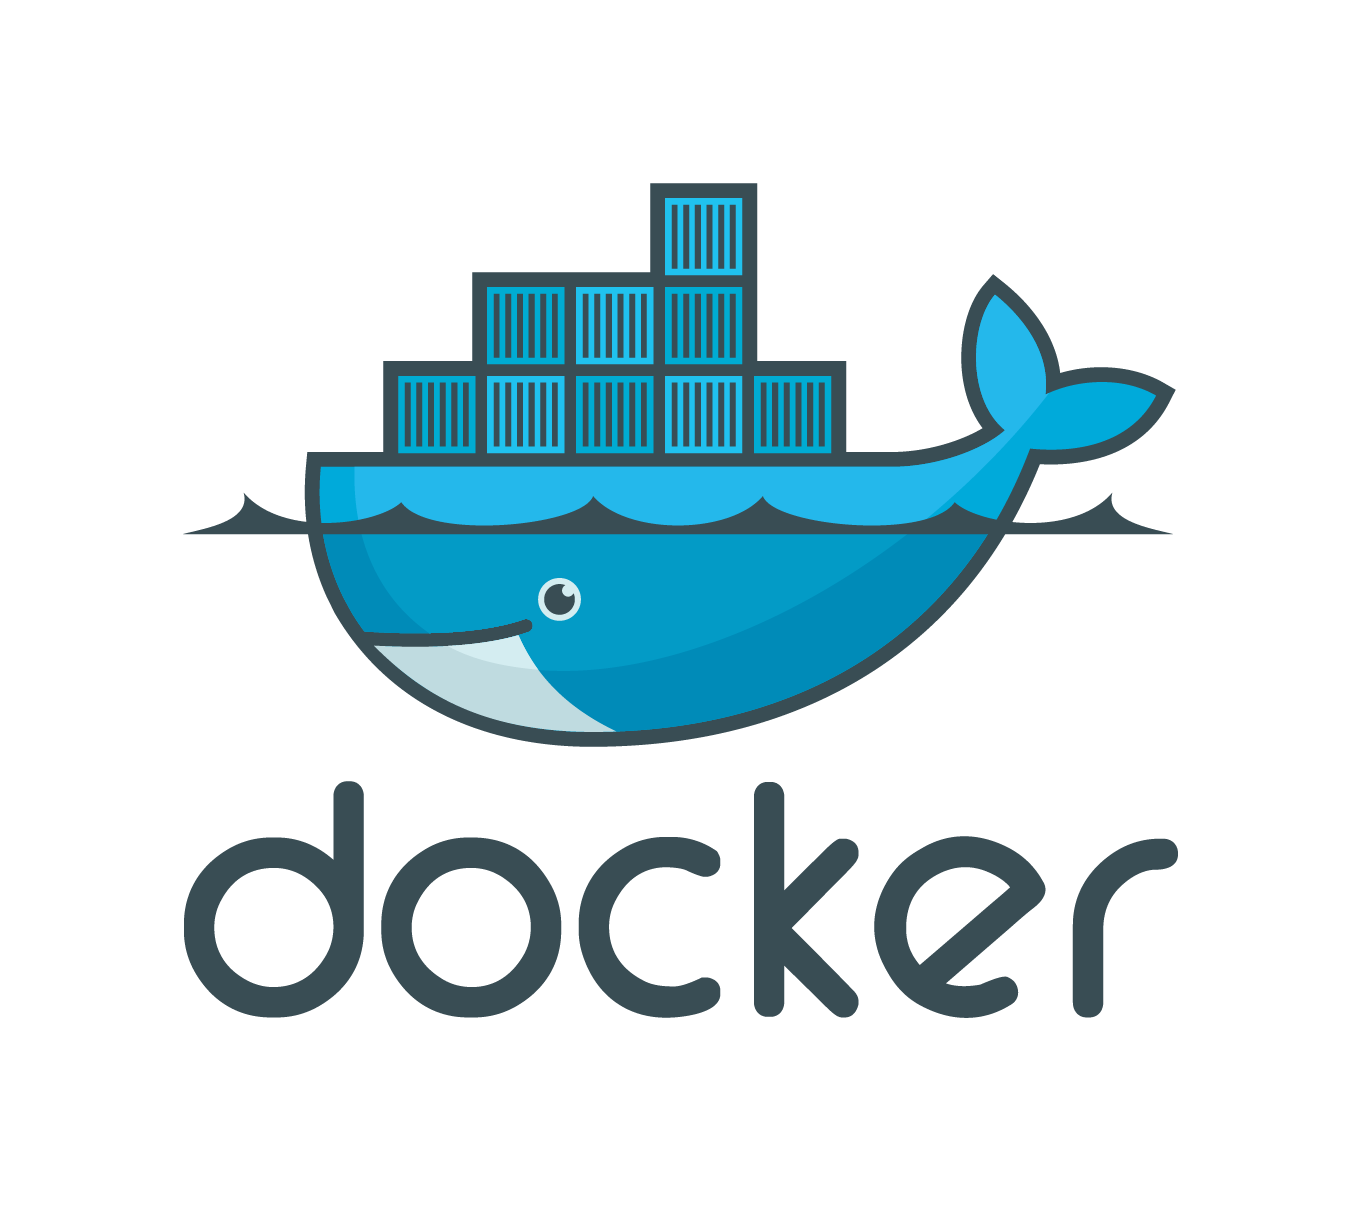
\includegraphics[scale=0.30]{docker-logo.png}
            \caption{Logo de \docker{} - los contenedores que transportan mercadería en barcos representan el mismo concepto de estandarización que los contenedores \docker{}}
        \end{figure}

        \docker{} también permite \textbf{apilar} los contenedores, logrando armar el deseado para la aplicación a correr en base a una construcción de distintos contenedores previamente definidos. También permite hacer un gestionado de versiones de las distintas imágenes que se pueden crear, pudiendo así revertir cambios hechos a una imagen.
        
        \subsubsection*{\docker{} es como la \textit{JVM}}
            \begin{quote}
                Promesa de Java: \textit{Escribir una vez. Ejecutar en todos lados.}
            \end{quote}

            En vez del código el que debe ser escrito una vez y poder ser ejecutado en todos lados, las plataformas de contenedores plantean una solución similar pero del lado de la configuración del servidor. Con los contenedores, los desarrolladores pueden tener la confianza que su plantilla de servidor correrá igual en todos los anfitriones donde se ejecute una plataforma de contenedores.\cite{ctl}

        \subsubsection*{\docker{} es como \textit{Git}}
            \begin{quote}
                Promesa de Git: \textit{Huellas minúsculas con rendimiento veloz.}
            \end{quote}

            Como se decía anteriormente, \docker{} permite hacer un seguimiento de las distintas versiones por las que pasó una imagen (en vez de seguir el código, como hace \textit{Git}).\cite{ctl}

        \subsection{¿Qué \textbf{NO} es \docker{}?}
        A primera vista, \docker{} se puede pensar como ``máquinas virtuales livianas''. Este concepto no es acertado, debido a que, como se explicó anteriormente, las máquinas virtuales difieren de las plataformas de contenedores en su forma de abstraer los recursos y de presentar esa abstracción al usuario.

        \begin{enumerate}
            \item \docker{} no es una tecnología de contenedores Linux (como LXC).
            \item \docker{} no es un reemplazo para un administrador de configuraciones (como pueden ser Chef, Pupper, SaltStack).
            \item \docker{} no es una \textit{Plataforma como Servicio} (PaaS).\cite{ctl}
        \end{enumerate}
    \subsection{Arquitectura}
        La plataforma \docker{} emplea los siguientes conceptos para describir su funcionamiento y arquitectura: 

        \begin{enumerate}
            \item \textbf{Imagen}: definición o plantilla del servidor el cual se virtualizará. Se definen qué dependencias debe tener la imagen.
            \item \textbf{Contenedor}: instancia de una imagen. Un contenedor corre una imagen en particular.
            \item \textbf{\docker{} Daemon}: procesos que corre en segundo plano y se encarga de administrar los distintos contenedores que se encuentren corriendo en un momento dado.
            \item \textbf{Dockerfile}: archivo que define la configuración que va a tener una imagen. Emplea una sintaxis específica para su escritura
            \item \textbf{\docker{} Compose}: herramienta que permite definir y correr simultáneamente varios contenedores. También permite crear un archivo de configuración para definir qué imágenes correr.
            \item \textbf{Local Registry}: repositorio en una red local de la cual los distintos clientes podrán descargar las imágenes que éste publica.
            \item \textbf{DockerHub}: sitio web que permite subir los repositorios de imágenes y de esta manera se pueden compartir entre distintos usuarios de manera globa.
        \end{enumerate}
        

    \clearpage
    \section{Ventajas y desventajas}
        \subsubsection*{Ventajas}
        Como ya se fue diciendo a lo largo de este trabajo, tanto \docker{} como las plataformas de contenedores en general ofrecen varias ventajas sobre las máquinas virtuales u otras técnicas de virtualización. La principal de ellas es que los contenedores son más \textbf{livianos} que las máquinas virtuales, permitiendo así poder crear varios a la vez y ejecutarlos en simultáneo. También brinda grandes posibilidades de abstracción de la aplicación a correr, logrando tener distintos contenedores, aislados entre sí, pero que entre todos ofrecen la posibilidad de montar una aplicación.

        \begin{figure}[h]
            \centering
            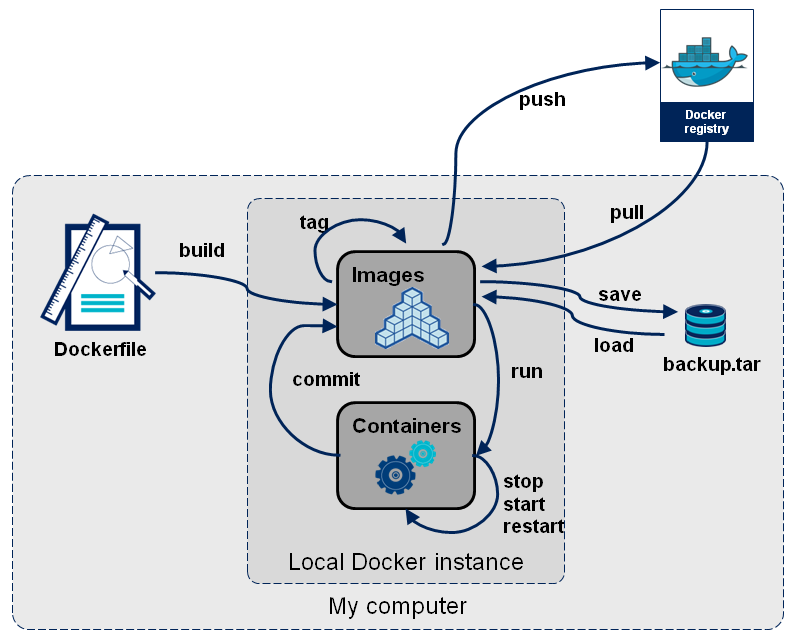
\includegraphics[scale=0.65]{docker-stages.png}
            \caption{Interacción entre los distintos elementos de la arquitectura de \docker{}\cite{stages}}
        \end{figure}

        La \textit{API} que ofrece \docker{} también es muy sencilla, siendo muy intuitivo si ya se cuenta con experiencia en otras herramientas como \textit{Git}

        Una de las ventajas más importantes que brinda \docker{} que no se debe dejar de lado es la facilidad con la cual los desarrolladores pueden mover su aplicación entre distintos servidores que corran la plataforma, manteniendo así la independencia del hardware.

        
        \subsubsection*{Desventajas}
        Más allá de los distintos beneficios y nuevas posibilidades que brindan los contenedores frente a las máquinas virtuales, esta técnica de virtualización también se enfrenta con varias dificultades, siendo uno de los mayores problemas la \textbf{incompatibilidad entre distintos sistemas operativos} y la \textbf{seguridad}.

        Como los contenedores se basan en el sistema operativo anfitrión, utilizan su mismo filesystem para los distintos contenedores que corra la plataforma. Este aspecto es uno de los que brinda las mayores ventajas, ya que es el que evita tener que virtualizar todo el hardware. Sin embargo, imposibilita correr una imagen de un sistema operativo que utilice un filesystem distinto al del sistema operativo anfitrión. Por ejemplo, no se puede correr una imagen de un sistema operativo Linux (ext4) en una máquina con Windows (NTFS).
        Con respecto a los problemas con la seguridad, vienen dados por una situación: \textbf{el demonio de \docker{} siempre corre con privilegios de superusuario}. Según la documentación oficial de la herramienta \cite{docs}, esto sucede porque el proceso demonio se conecta con un socket Unix en vez de con un socket TCP. Por defecto dicho socket Unix es propiedad del usuario \textit{root}. Además, los procesos dentro de los contenedores se ejecutan, por defecto, con permisos de superusuario.

        Estas dos características que tiene por defecto \docker{} pueden ser problemáticas al momento de que el proceso con permisos de superusuario del contenedor se comunique con el kérnel (que es el mismo kérnel de la máquina anfitrión, porque comparte el sistema operativo).  

        Una regla básica que se intenta mantener es la de \textit{tratar a los contenedores del mismo modo que se trataría a cualquier servidor de aplicación}. Esto significa:
        \begin{enumerate}
            \item Remover privilegios cuanto antes
            \item Correr los servicios del contenedor sin permisos de superusuario siempre que sea posible
            \item Tratar al usuario \textit{root} del contenedor como si fuera el usuario \textit{root} de la máquina anfitrión \cite{walsh}
        \end{enumerate}




    \clearpage
    \section{Ejemplo práctico}


    \clearpage
    \bibliographystyle{plainnat}
    \bibliography{tp_final}

\end{document}
